\begin{center}
\begin{longtable}{ |l|l| } 
 \hline
 Attribute & Description\\ 
 \hline
 timestamp & when ad was clicked\\ 
 \hline
 txId & ID of the click\\ 
 \hline
 userSessionId & ID of the users session who made the click\\ 
 \hline
 teamId & ID of the team that user is in\\ 
 \hline
 userId & ID of the user that made the click\\ 
 \hline
 adId & ID of an add that was clicked\\ 
 \hline
 adCategory & type of an ad that was clicked\\ 
 \hline
\caption{ad-clicks.csv}
\end{longtable}
\end{center}

Inspecting for missing data in adClicks showcases no missing values.
\begin{figure}[H]
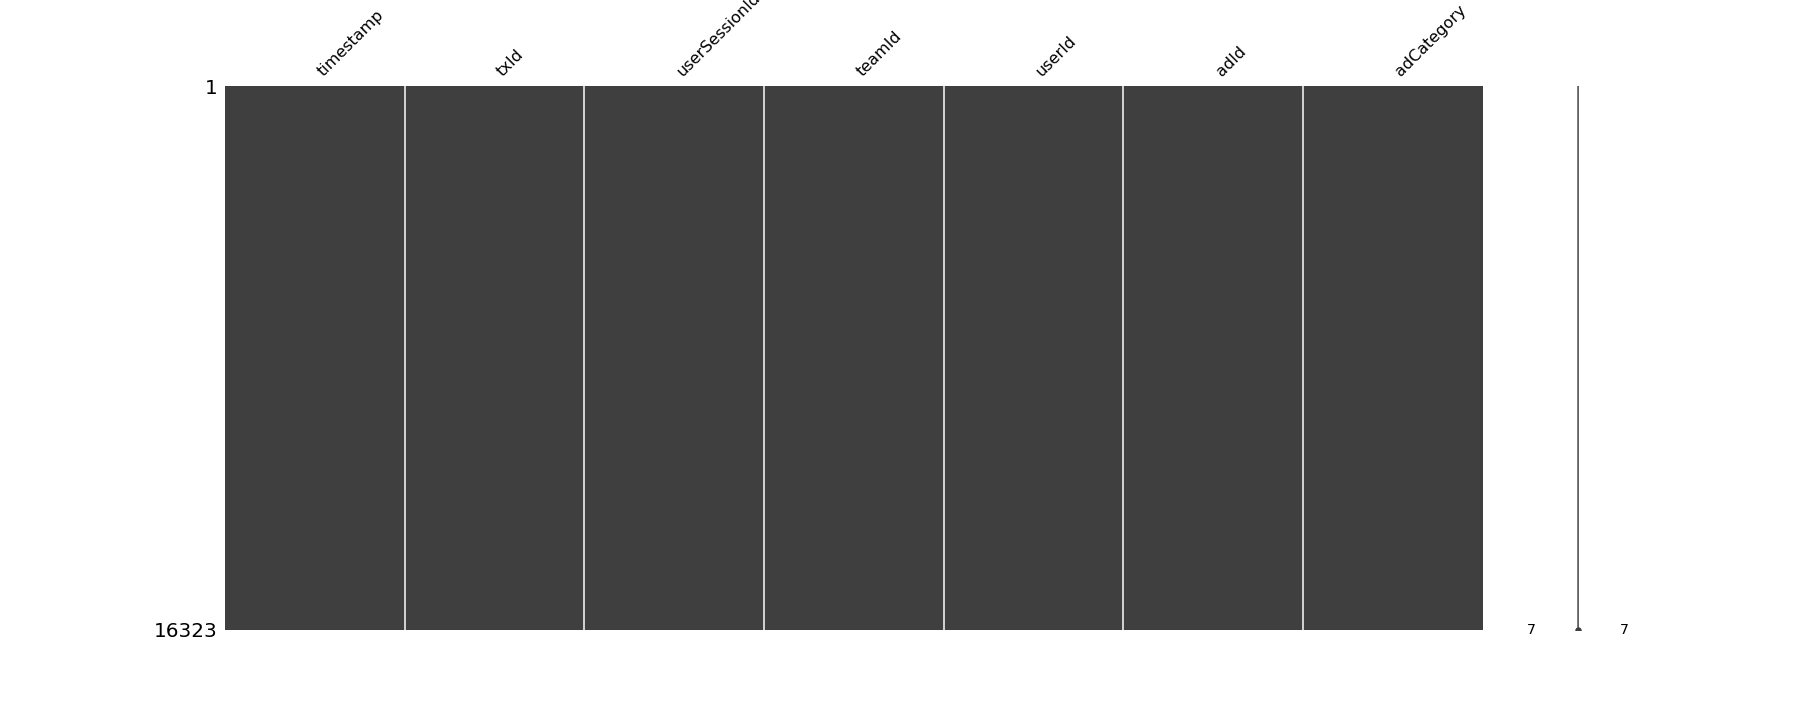
\includegraphics[scale=0.25]{img/Graphs/adClicks/missingno_adClicks.png}
\centering
\caption{adClicks\_msno}
\label{fig:adClicks_msno}
\end{figure}

Figure (ID) represents decline of ad clicks over time. From business point of view, decline looks steep and fast, therefore something must have happened with the game.
\begin{figure}[H]
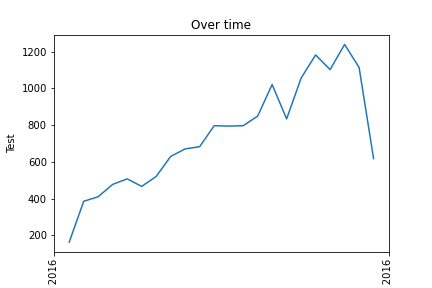
\includegraphics[scale=0.85]{img/Graphs/adClicks/timeseries_adClicks.png}
\centering
\caption{timeseries\_adClicks}
\label{fig:timeseries_adClicks}
\end{figure}

Looking at the biggest teams, we can see that team with id 64 has occurred 681 times. With knowing what top teams are doing, we can assume other teams will copy them.
\begin{figure}[H]
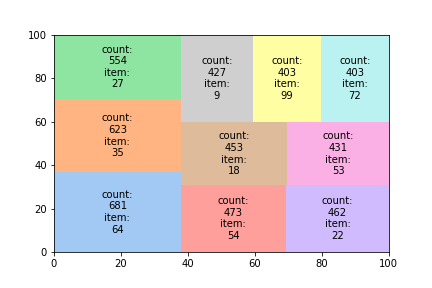
\includegraphics[scale=0.85]{img/Graphs/adClicks/tree_map_adClicks.png}
\centering
\caption{adClicks\_tree\_map}
\label{fig:adClicks_tree_map}
\end{figure}

Comparing IDs of ads to the sections they are representing, we can see that computers and games have the most IDs. This would make sense since the product we are offering is computer game. Other products have on average 3 IDs meaning they aren't so popular.
\begin{figure}[H]
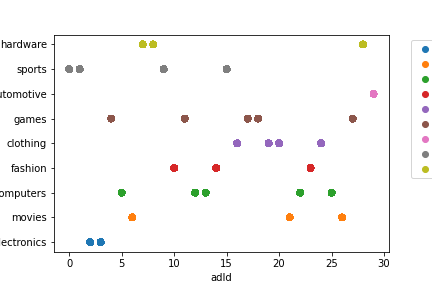
\includegraphics[scale=0.85]{img/Graphs/adClicks/create_ad_adClicks.png}
\centering
\caption{adClicks\_create\_ad}
\label{fig:adClicks_create_ad}
\end{figure}